\section{Subsystem decomposition}

We have chosen to use the MVC design pattern, to make a clear distinction of what functionality 
should be assigned to which part of our system. The MVC pattern stands for Model-View-Control, 
and it’s commonly used for implementing user interfaces.
\\\\
We have also chosen to create a database, whereas this database will be used to store persistent data, to when the user will logout or close the program. This will make it possible to receive earlier used data.

As we have chosen to use the MVC pattern, we will have 3 different subsystems, plus the subsystem of our database storage:

\begin{itemize}
	\item Model
	\item View
	\item Control
	\item DataStorage
\end{itemize}

Our \textbf{Model subsystem} has the responsibility to keep notifying the controllers to update the views, which the user is using. Here is a picture of our subsystem:\\
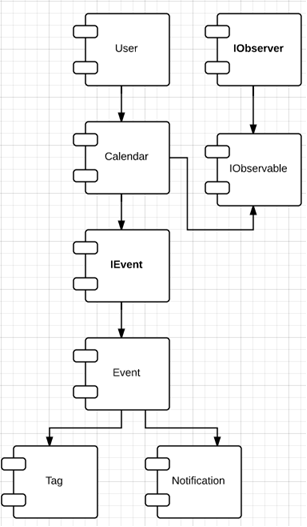
\includegraphics[scale=0.8]{modelSubsystem}

\pagebreak

Our \textbf{View subsystem} has the responsibility to represent the model’s state. Whenever the state of the model is changed, the view will also be changed to represent the new state of the model. Here is a picture of our subsystem:\\
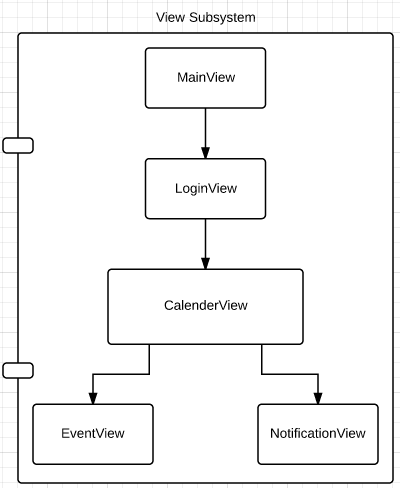
\includegraphics[scale=0.8]{viewSubsystem}
\\

Our \textbf{Control subsystem} has the responsibility to update the view, whenever the model has changed. The controllers will be used to update the views, by being notified by the model about its state. Here is a picture of subsystem:\\
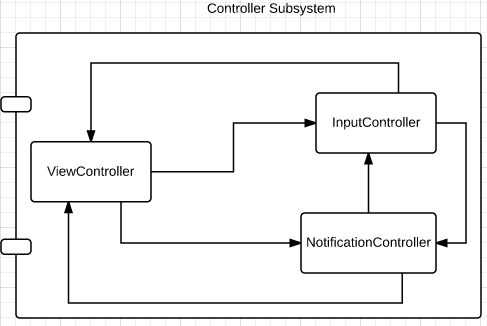
\includegraphics[scale=0.8]{controlSubsystem}

\pagebreak

Our \textbf{DataStorage subsystem} has the responsibility to save persistent data, which the system will be using at another time. Persistent data could be a calendar for a specific user. When the user will be login into the system, the controllers will be using the DataStorage subsystem to receive the calendar. Here is a picture of our subsystem:\\
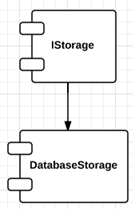
\includegraphics[scale=0.8]{datastorageSubsystem}